\chapter{Fourier transforms of tempered distributions and
  applications}\label{chap4}

\setcounter{pageoriginal}{0}
\section*{Fourier transforms of $L^{1}$ functions}\pageoriginale

Let $x=(x_{1},\ldots,x_{n})$ and $\xi=(\xi_{1}\ldots\xi_{n})$ be
elements of $\mathbb{R}^{n}$. We denote by $x$, $\xi$ the number
$\sum\limits^{n}_{j=1}x_{j}\xi_{j}$. 

If $f\in L^{1}(\mathbb{R}^{n})$ (with respect to the Lebesgue measure)
we define the Fourier transform $f$ of by:
$$
\widehat{f}(\xi)=\int\limits_{\mathbb{R}^{n}}e^{-2\pi
  ix.\xi}f(x)dx,\quad\text{where}\quad i=\sqrt{-1}.
$$
Sometimes we also denote $\widehat{f}$ by $\mathfrak{F}(f)$.

\begin{exer*}
Prove that $\widehat{f}$ is a continuous bounded function and
$\displaystyle{\mathop{\Sup}\limits_{\xi\in \mathbb{R}^{n}}}\;|\widehat{f}(\xi)|\leq ||f||_{L^{1}}$.
\end{exer*}

\setcounter{proposition}{0}
\begin{proposition}\label{chap4-prop1}
Let $f\in L^{1}(\mathbb{R}^{n})$. For $h\in \mathbb{R}^{n}$ denote by
$\tau_{h}f$ the function $x\mapsto f(x-h)$. We have
\begin{itemize}
\item[\rm(i)] $\mathfrak{F}(\tau_{h}f)=e^{-2\pi ih\cdot
  \xi}\mathfrak{F}(f)$

\item[\rm(ii)] $\tau_{h}\widehat{f}=\mathfrak{F}(e^{2\pi ih\cdot x}f)$

\item[\rm(iii)] If $f$ and $g$ belong to $L^{1}$ then $f\ast g$
  belongs to $L^{1}$ and $\mathfrak{F}(f\ast g)=\mathfrak{F}(f)\cdot
  \mathfrak{F}(g)$

\item[\rm(iv)] If $\psi(x)=f(x/\lambda)$, $\lambda >0$, then $\widehat{\psi}(\xi)=\lambda^{n}\widehat{f}(\lambda,\xi)$.
\end{itemize}
\end{proposition}

\begin{remark*}
The crucial property of Fourier transform is that it converts
convolution product into ordinary pointwise product (property iii in
the proposition).
\end{remark*}

\begin{proof}
\begin{itemize}
\item[\rm(i)]\pageoriginale
\begin{tabbing}
\,\qquad\quad$\mathfrak{F}(\tau_{h}f)(\xi)$ \== $\int e^{-2\pi
    ix.\xi}f(x-h)dx$\\[3pt]
\>= $\int e^{-2\pi i(y+h)\xi}f(y)dy$\quad (put $x-h=y$)\\[3pt]
\>= $e^{-2\pi ih \xi}\widehat{f}(\xi)$.
\end{tabbing}

(3) If $f$, $g\in L^{1}$, the function $f(x-y)g(y)$ is measurable in
$\mathbb{R}^{n}\times \mathbb{R}^{n}$ and so is the function
$|f(x-y)g(y)|$. Moreover $\int |f(x-y)|dx=\int  |f(x)|dx$. Thus the
repeated integral $\int |g(y)|(\int |f(x-y)|dx)dy$ exists. Hence by
Fubini's theorem $|f(x-y)g(y)|$ is integrable in $\mathbb{R}^{n}\times
  \mathbb{R}^{n}$ and $x\mapsto \int f(x-y)g(y)dy$ is integrable.

Put $h(x)=\int f(x-y)g(y)dy$. Using Fubini's theorem we see that
\begin{align*}
\widehat{h}(\xi) &= \int e^{-2\pi ix\xi}\{f(x-y)g(y)dy\}dx\\[3pt]
&= \int g(y)\left\{\int e^{-2\pi i \xi x}f(x-y)dx\right\}dy\\[3pt]
&= \int g(y)\mathfrak{F}(\tau_{y}f)dy\\[3pt]
&= \int g(y)e^{-2\pi iy\xi}\widehat{f}(\xi)\; dy\quad \text{~~ (by
  i)}\\[3pt]
&= \widehat{f}(\xi)\widehat{g}(\xi).
\end{align*}
(ii) and (iv) are left as exercises.
\end{itemize}
\end{proof}

\begin{exer*}
Show that the convolution in $L^{1}(\mathbb{R}^{n})$ is commutative
and associative. Moreover if $f$, $g\in L^{1}$, $||f\ast
g||_{L^{1}}\leq ||f||_{L^{1}}||g||_{L^{1}}$. Thus
$L^{1}(\mathbb{R}^{n})$ is a commutative Banach algebra under convolution.
\end{exer*}

\section*{The Schwartz space of rapidly decreasing functions}

A complex valued function $f$ on $\mathbb{R}^{n}$ is said to be
rapidly decreasing if $f$ is $C^{\infty}$ and $\lim\limits_{|x|\to
  \infty}|x|^{k}|D^{\alpha}f(x)|=0$ for every integer $k\geq 0$ and
every multi-index $\alpha$. Thus $f$ and its derivatives decrease, as
$|x|\to \infty$, more rapidly than any power of $\dfrac{1}{|x|}$.

If\pageoriginale $f$ is $C^{\infty}$, the above condition is
equivalent to each of the following conditions.
\begin{itemize}
\item[(a)] For any polynomial $P(x)=P(x_{1}\ldots x_{n})$ and any
  linear differential operator $L$ with constant coefficients, the
  function $P(Lf)$ is bounded in $\mathbb{R}^{n}$.

\item[(b)] With the above notation $L(Pf)$ is bounded in
  $\mathbb{R}^{n}$.

\item[(c)] For all $k\geq 0$ and $\alpha |(1+|x|^{2})^{k}D^{\alpha}f|$
  is bounded in $\mathbb{R}^{n}$.
\end{itemize}

This is seen by using Leibniz formula and

\begin{exer*}
Let $k\geq 0$ be an integer. Then there exist constants $M_{1}$ and
$M_{2}$, depending only on $k$ and $n$, such that, for all $\xi\in
\mathbb{R}^{n}$, we have
$$
M_{2}(1+|\xi|^{2})^{k/2}\leq \sum\limits_{|\alpha|\leq
  k}|\xi^{\alpha}|\leq M_{1}(1+|\xi|^{2})^{k/2}.
$$
Also there exist constants $C_{1}$ and $C_{2}$ such that for all $\xi
\in \mathbb{R}^{n}$ we have
$$
C_{2}(1+|\xi|^{2})^{k}\leq \sum\limits_{|\alpha|\leq
  k}|\xi^{\alpha}|^{2}\leq C_{1}(1+|\xi|^{2})^{k}.
$$

We shall denote by $\mathfrak{I}$ the vector space of rapidly
decreasing functions and call it the Schwartz space (or
$\mathbb{R}^{n}$). We shall say that a sequence $\{f_{k}\}$ in
$\mathfrak{I}$ tends to zero in $\mathfrak{I}$, if for every
polynomial $P$ in $(x_{1},\ldots,x_{n})$ and linear differential
operator $L$ with constant coefficients (in $\mathbb{R}^{n}$), the
sequence $P(L(f_{k}))$ tends to zero uniformly in $\mathbb{R}^{n}$. A
linear map $F:\mathfrak{I}\to \mathfrak{I}$ (or $\mathfrak{I}\to
\mathbb{C}$) will be said to be continuous if for $f_{k}\to 0$ in
$\mathfrak{I}$ we have $F(f_{k})\to 0$ in $\mathfrak{I}$ (or in $\mathbb{C}$).
\end{exer*}

\begin{proposition}\label{chap4-prop2}
If $f$ is an element in $\mathfrak{I}$ then $f$ belongs to
$L^{1}$. Moreover if $f_{n}\to 0$ in $\mathfrak{I}$, then $f_{n}\to 0$
in $L^{1}$.
\end{proposition}

\begin{proof}
We have for every non-negative integer $k$ a positive constant $M$
with $(1+|x|^{2})^{k}|f(x)|\leq M$ or $|f(x)|\leq M/(1+|x|^{2})^{k}$
for $x\in \mathbb{R}^{n}$. But\pageoriginale the function
$(1+|x|^{2})^{k}$ is summable in $\mathbb{R}^{n}$ if $k>n/2$, as is
seen by using polar coordinates: $dx=r^{n-1}dr \ d\Omega$. Choosing
$k>n/2$ we see that $f$ is in $L^{1}$. Moreover for such a choice of
$k$ we have
\begin{align*}
\int |f_{k}(x)|dx &= \int
(1+|x|^{2})^{k}|f_{k}|\frac{1}{(1+|x|^{2})^{k}}dx\\[3pt]
&\leq \sup\limits_{x\in \mathbb{R}^{n}}\left((1+|x|^{2})^{k}|f_{k}(x)|\right)\int\dfrac{dx}{(1+|x|^{2})^{k}}.
\end{align*}
This proves the second part of the proposition.
\end{proof}

\begin{exer*}
With the above notation, prove that if $f\in \mathfrak{I}$, then
$P(L(f))$ belongs to $\mathfrak{I}$ and that the linear map $f\mapsto
P(L(f))$ from $\mathfrak{I}$ to $\mathfrak{I}$ is continuous.
\end{exer*}

\begin{exer*}
Prove that if $f\in \mathfrak{I}$, then $f$ belongs to $L^{p}$ for
$p\geq 1$ and that the inclusion $\mathfrak{I}\to L^{p}$ is ``continuous''.
\end{exer*}

Note that $\mathcal{D}$ is contained in $\mathfrak{I}$.

\begin{proposition}\label{chap4-prop3}
$\mathcal{D}$ is dense in $\mathfrak{I}$. That is, given $f\in
  \mathfrak{I}$, there exists a sequence $\{\varphi_{k}\}$ in
  $\mathcal{D}$ such that $\varphi_{k}-f$ tends to zero in $\mathfrak{I}$.
\end{proposition}

\begin{proof}
Let $\Psi_{k}$ be a sequence in $\mathcal{D}$ such that for any
multi-index $\alpha$ we have
\begin{enumerate}
\renewcommand{\labelenumi}{(\theenumi)}
\item $D^{\alpha}(\Psi_{k}-1)$ tends to zero uniformly on compact sets

\item $D^{\alpha}(\Psi^{k}-1)$ are uniformly bounded in $x$ and
  $k$. (we can take for $\Psi_{k}$ the function
  $\Psi_{k}(x)=\eta\left(\dfrac{x}{k}\right)$, where $\eta\in
  \mathcal{D}(\mathbb{R}^{n})$ with $\eta(x)=1$ for $|x|\leq 1$). It
  is easy to see that $\Psi_{k}f-f$ tends to zero in
  $\mathfrak{I}$. In fact, by Leibniz formula,
$$
PD^{\alpha}\{(1-\Psi_{k})f\}=\sum\limits_{\beta\leq
  \alpha}C_{\alpha,\beta}D^{\beta}(1-\Psi_{k}). P.D^{\alpha-\beta}
$$
for any polynomial $P$, where $C_{\alpha,\beta}$ are constants
depending only on $\alpha$\pageoriginale and $\beta$. Since $f\in
\mathfrak{I}$, $PD^{\alpha-\beta}f$ tends to zero at infinity, so that
it can be made arbitrarily small in the complement of compact
sets. Using $D^{\beta}(1-\Psi_{k})$ is bounded in $x$ and $k$ and
$D^{\beta}(1-\Psi_{k})$ tends to zero on compact sets, we see that
$\Psi_{k}f\to f$ in $\mathfrak{I}$.
\end{enumerate}
\end{proof}

\section*{Fourier transforms in $\mathfrak{I}$.}

If $f\in \mathfrak{I}$, then by Proposition \ref{chap4-prop2}, $f$
belongs to $L^{1}$ and hence the Fourier transform of $f$ is defined.

\begin{proposition}\label{chap4-prop4}
The Fourier transform maps $\mathfrak{I}$ into itself. Moreover for
$f\in \mathfrak{I}$ we have
\begin{itemize}
\item[\rm(i)] $\mathfrak{F}(D^{\alpha}f)=(2\pi i
  \xi)^{\alpha}\mathfrak{F}(f)$ \ and

\item[\rm(ii)] $D^{\alpha}\widehat{f}=\mathfrak{F}((-2\pi i)^{|\alpha|}x^{\alpha}f)$.
\end{itemize}
More generally, if $P$ is a polynomial $\sum\limits_{|\alpha|\leq
  m}a_{\alpha}D^{\alpha}$ and $P(D)=\sum\limits_{|\alpha|\leq
  m}a_{\alpha}D^{\alpha}$ the corresponding differential operator,
then
\begin{align*}
\mathfrak{F}(P(D)f) &= P(2\pi
i\xi)\mathfrak{F}(f)\quad\text{and}\\[3pt]
P(D)\widehat{f} &= \mathfrak{F}(P(-2\pi ix)f).
\end{align*}
\end{proposition}

\begin{proof}
Let $f\in \mathfrak{I}$. We have
$$
\widehat{f}(\xi)=\int e^{-2\pi ix\xi}f(x)dx.
$$
We shall first show that $\widehat{f}$ is $C^{\infty}$. Since
$$
\dfrac{\partial}{\partial \xi_{j}}\left(e^{-2\pi ix
  \xi}f(x)\right)=(-2\pi ix_{j})e^{-2\pi ix\xi}f(x)
$$
is integrable and is dominated by the integrable function $2\pi
x_{j}f$ independent of $\xi$, we see that $f$ is differentiable and
\begin{align*}
\frac{\partial \widehat{f}}{\partial \xi_{j}} &= \int e^{-2\pi
  ix\xi}(-2\pi ix_{j})f(x)dx\\[4pt]
&= \mathfrak{F}(-2\pi ix_{j}f).
\end{align*}
Inductively we see that $f$ is $C^{\infty}$ and
$$
D^{\alpha}\widehat{f}=\mathfrak{F}((-2\pi ix)^{\alpha}f).
$$\pageoriginale
(It is thus the rapid decrease of $f$ at infinity which assures that
$\widehat{f}$ is $C^{\infty}$).

Next we show that $f$ is rapidly decreasing. Let us first look at the
case $n=1$. Noting that the Fourier transform of a function in $L^{1}$
is bounded and using induction, it is enough the show that
\begin{align*}
2\pi i\xi \widehat{f}(\xi) &= \int e^{-2\pi
  ix\xi}f'(x)dx.\quad\text{Now}\\[4pt]
(2\pi i\xi)\widehat{f}(\xi) &= \lim\limits_{\ell \to
  \infty}\int\limits^{\ell}_{-\ell}2\pi i\xi. e^{-2\pi
  ix\xi}f(x)dx\\[4pt]
&= \lim\limits_{\ell\to
  \infty}\int\limits^{\ell}_{-\ell}-\dfrac{d}{dx}(e^{-2\pi
  ix\xi})f(x)dx\\[4pt]
&= \lim\limits_{\ell \to
  \infty}\left\{\int\limits^{\ell}_{-\ell}e^{-2\pi
  ix\xi}f'(x)dx-\left[e^{-2\pi
    ix\xi}f(x)\right]^{\ell}_{-\ell}\right\}\\[4pt]
&= \int\limits_{\mathbb{R}}e^{-2\pi ix\xi}f'(x)dx
\end{align*}
(Thus the fact that the successive derivatives are summable implies
the rapid decrease of $f$ at infinity. Thus there is an exchange
between these two properties). Now consider the case of
$\mathbb{R}^{n}$, $n\geq 2$. It is enough to show that
$$
\mathfrak{F}\left(\frac{\partial f}{\partial x_{j}}\right)=2\pi i\xi_{j}\mathfrak{F}(f).
$$
If $x=(x_{1},\ldots,x_{j},\ldots,x_{n})$, we write
$x'=(x_{1},\ldots,x_{j-1},x_{j+1},\ldots,x_{n})$ and
$x=(x',x_{j})$. By Fubini's theorem, for almost all $x'\in
\mathbb{R}^{n-1}$, the functions $x_{j}\mapsto f(x',x_{j})$ and
$x_{j}\mapsto \dfrac{\partial f}{\partial x_{j}}(x',x_{j})$ are
integrable over $\mathbb{R}$. By integrating by parts and passing to
the limit as $\ell\to \infty$, as above, we obtain
$$
\int\limits^{\infty}_{-\infty}e^{-2\pi ix\xi}\dfrac{\partial
  f}{\partial x_{j}}dx_{j}=2\pi
i\xi_{j}\int\limits^{\infty}_{-\infty}e^{-2\pi ix\xi}f(x)dx_{j},
$$
for\pageoriginale almost all $x'\in \mathbb{R}^{n-1}$. By applying
Fubini's theorem and integrating with respect to $x'$ we get
$$
\mathfrak{F}\left(\dfrac{\partial f}{\partial x_{j}}\right)=2\pi i\xi_{j}\mathfrak{F}(f).
$$
\end{proof}

\begin{proposition}\label{chap4-prop5}
The maps $f\mapsto \mathfrak{F}(f)$ is a continuous linear map from
$\mathfrak{I}$ to $\mathfrak{I}$.
\end{proposition}

\begin{proof}
By Proposition \ref{chap4-prop3} we have
$$
\xi^{\beta}D^{\alpha}\mathfrak{F}(f)=(2\pi i)^{|\alpha|-|\beta|}\int
e^{-2\pi ix\xi}D^{\beta}((-x)^{\alpha}f(x))dx.
$$
If $f_{k}\to 0$ in $\mathfrak{I}$, then
$D^{\beta}((-x)^{\alpha}f_{k})\to 0$ in $\mathfrak{I}$ (see the
Exercise following Proposition \ref{chap4-prop2}) and hence, by
Proposition \ref{chap4-prop2},
\begin{align*}
& ||D^{\beta}((-x)^{\alpha}f_{k})||_{L^{1}}\to
  0.\quad\text{But}\\[3pt]
& \Sup\limits_{\xi\in
    \mathbb{R}^{n}}|\xi^{\beta}D^{\alpha}\mathfrak{F}(f_{k})|\leq
  \text{Const. } ||D^{\beta}((-x)^{\alpha}f_{k})||_{L^{1}}
\end{align*}
and hence tends to zero as $k\to \infty$.
\end{proof}

\section*{Fourier inversion theorem.}

\setcounter{theorem}{0}
\begin{theorem}\label{chap4-thm1}
Let $g\in \mathfrak{I}$. Then
$$
g(x)=\int\limits_{\mathbb{R}^{n}}e^{-2n i \xi x}\widehat{g}(\xi)d\xi
$$
for $x\in \mathbb{R}^{n}$.
\end{theorem}

First we prove

\setcounter{lemma}{0}
\begin{lemma}[Weak Parseval relation]\label{chap4-lem1}
Let $f$, $g\in \mathfrak{I}$. Then we have
$$
\int f(x)\widehat{g}(x)dx=\int \widehat{f}(\xi)g(\xi)d\xi.
$$
\end{lemma}

\begin{proof}
We have, by Fubini's theorem,
\begin{align*}
\int f(x)\widehat{g}(x)dx &= \iint f(x)e^{-2\pi ix\xi}g(\xi)d\xi
dx\\[3pt]
&= \int g(\xi)\left(\int f(x)e^{-2\pi ix\xi}d\xi\right)d\xi\\[3pt]
&= \int g(\xi)\widehat{f}(\xi)d\xi.
\end{align*}\pageoriginale
\end{proof}

\noindent
{\bf Proof of Theorem \ref{chap4-thm1}.}~
For $\varphi\in \mathfrak{I}$ and $\lambda >0$, put
$f(x)=\varphi(x/\lambda)$. Then by Proposition \ref{chap4-prop1},
(iv), we have $\widehat{f}(\xi)=\lambda^{n}\widehat{\varphi}(\lambda
\xi)$. By the above Lemma \ref{chap4-lem1} we obtain
\begin{align*}
& \int g(\xi)\lambda^{n}\widehat{\varphi}(\lambda \xi)d\xi=\int
  \varphi\left(\frac{x}{\lambda}\right)\widehat{g}(x)dx\quad\text{or}\\[3pt]
& \int g(\xi/\lambda)\widehat{\varphi}(\xi)d\xi=\int \varphi (x/\lambda)\widehat{g}(x)dx.
\end{align*}
As $\lambda\to \infty$, $g(\xi/\lambda)\to g(0)$ and
$\varphi(x/\lambda)\to \varphi(0)$. Moreover
$\displaystyle{\mathop{\Sup}_{\xi}}|g(\xi/\lambda)|=\displaystyle{\mathop{\Sup}_{\xi}}|g(\xi)|=M<\infty$'
hence $|g(\xi/\lambda)\widehat{\varphi}(\xi)|\leq
M|\widehat{\varphi}(\xi)|$. Similarly
$$
|\varphi (x/\lambda)\widehat{g}(x)|\leq
\left(\displaystyle{\mathop{\Sup}_{y}}|\varphi (y)|\right)|\widehat{g}(x)|.
$$
Hence we may apply the dominated convergence theorem to conclude that
$$
g(0)\int \widehat{\varphi}(\xi)d\xi=\varphi(0)\int \widehat{g}(x)dx.
$$
We shall prove in the next proposition that there exists $\varphi\in
\mathfrak{I}$ with $\varphi(0)=1$ and $\int
\widehat{\varphi}(\xi)d\xi=1$. We thus obtain
$$
g(0)=\int \widehat{g}(x) dx,\quad\text{for}\quad g\in \mathfrak{I}.
$$
To get the value of $g$ at an arbitrary $x$ we note that
\begin{align*}
g(x) &= (\tau_{-x}g)(0)=\int \widehat{\tau_{-x}(g)}d\xi\\[3pt]
&= \int e^{2\pi ix\xi}\widehat{g}(\xi)d\xi,
\end{align*}
by Proposition \ref{chap4-prop1}, (i).

\begin{proposition}\label{chap4-prop6}
Let $\varphi(x)=e^{-\pi |x|^{2}}$. Then
$\widehat{\varphi}(\xi)=e^{-\pi|\xi|^{2}}$. Moreover\pageoriginale
$\varphi(0)=1$ and $\int \widehat{\varphi}(\xi)d\xi=1$.
\end{proposition}

We first prove

\begin{lemma}\label{chap4-lem2}
$\int\limits^{\infty}_{-\infty}e^{-\pi x^{2}}dx=1$.
\end{lemma}

\begin{proof}
\begin{align*}
\left(\int\limits^{\infty}_{-\infty}e^{-\pi x^{2}}dx\right)^{2} &=
\left(\int\limits^{\infty}_{-\infty}e^{-\pi
  x^{2}}dx\right)\left(\int\limits^{\infty}_{-\infty}e^{-\pi
  y^{2}}dy\right)\\[4pt]
&= \int\limits_{\mathbb{R}^{2}}e^{-\pi (x^{2}+y^{2})}dx \ dy\\[4pt]
&= \int\limits^{2\pi}_{0}\int\limits^{\infty}_{0}e^{-\pi r^{2}}\cdot
r\cdot dr \ d\theta\\[4pt]
&= \int\limits^{2\pi}_{0}d\theta\cdot \int\limits^{\infty}_{0}e^{-\pi
  r^{2}}\cdot r \ dr\\[4pt]
&= 2\pi \int\limits^{\infty}_{0}\dfrac{d}{dr}\left(-\frac{e^{-\pi
    r^{2}}}{2\pi}\right)dr\\[4pt]
&= 2\pi \left\{\frac{e^{-\pi r^{2}}}{2\pi}\right\}^{0}_{\infty}\\[4pt]
&= 2\pi/2 \pi=1.
\end{align*}
Since $\int\limits^{\infty}_{-\infty}e^{-\pi x^{2}}dx\geq 0$, we
obtain the Lemma.
\end{proof}

\noindent
{\bf Proof of Proposition \ref{chap4-prop6}.}~
The second part of the proposition holds since
$$
\int\limits_{\mathbb{R}^{n}}e^{-\pi|\xi|^{2}}d\xi
=\prod\limits^{n}_{j=1}
\left(\int\limits^{\infty}_{-\infty}e^{-\pi|\xi_{j}|^{2}}d\xi_{j}\right)=1,\qquad\text{by Lemma.}
$$
To prove the first part it is sufficient to consider the case $n=1$,
as
$$
\int\limits_{\mathbb{R}^{n}}e^{-2\pi ix\xi}e^{-\pi
  |x|^{2}}dx=\prod\limits^{n}_{j=1}\int\limits_{\mathbb{R}}e^{-2\pi ix_{j}\xi_{j}}e^{-\pi|x_{j}|^{2}}dx_{j}.
$$\pageoriginale
Now, taking $n=1$,
\begin{align*}
\int\limits_{\mathbb{R}}e^{-2\pi ix\xi}e^{-\pi x^{2}}dx &=
\int\limits_{\mathbb{R}}e^{-\pi (x^{2}+2ix\xi+(i\xi)^{2})-\pi
  \xi^{2}}dx\\[3pt]
&= e^{-\pi \xi^{2}}\int\limits_{\mathbb{R}}e^{-\pi (x+i\xi)^{2}}dx.
\end{align*}

To evaluate this integral for fixed $\xi$, consider in the complex
plane, the positively oriented rectangle formed by $-R$, $R$, $R+i\xi$
and $R-i\xi$.
\begin{figure}[H]
\centering
\includegraphics{chap4/1.eps}
\end{figure}

We shall apply Cauchy's theorem to the holomorphic function $e^{-\pi
  z^{2}}$ in this rectangle and let $R$ tend to infinity. Now if
$I(R)$ is the integral of $e^{-\pi z^{2}}$ on the vertical line from
$R$ to $R+i\xi$, we have
\begin{align*}
|I(R)| &= \left|\int\limits^{\xi}_{0}e^{-\pi
  (R+iy)^{2}} idy \right|\\[4pt]
&\leq \int\limits^{\xi}_{0}e^{-\pi R^{2}}e^{\pi y^{2}}dy\\[4pt]
&\leq \left(\int\limits^{\xi}_{0}e^{\pi y^{2}}dy\right)e^{-\pi
    R^{2}}\\[4pt]
&= C e^{-\pi R^{2}}
\end{align*}
where $C$ is a constant depending only on $\xi$ and not on $R$. Hence
$I(R)\to 0$ as $R\to \infty$. Thus the integrals on the vertical lines
tend to zero as $R\to \infty$. Hence
$$
\int\limits_{\mathbb{R}}e^{-\pi
  (x+i\xi)^{2}}dx=\int\limits_{\mathbb{R}}e^{-\pi
  x^{2}}dx=1\qquad\text{by Lemma \ref{chap4-lem2}.}
$$\pageoriginale
Thus
\begin{align*}
\int e^{-2\pi ix.\xi}e^{-\pi x^{2}}dx &= e^{-\pi \xi^{2}}\int e^{-\pi
  (x+i\xi)^{2}}dx\\[4pt]
&= e^{-\pi \xi^{2}}.
\end{align*}

\begin{proposition}\label{chap4-prop7}
The Fourier transform $\mathfrak{F}:\mathfrak{I}\to \mathfrak{I}$ is
an isomorphism. In fact it is a topological isomorphism in the sense
that $\mathfrak{F}$ and its inverse are continuous. The inverse is the
map $\overline{\mathfrak{F}}$ defined by $\overline{F}f(x)=\int
e^{2\pi ix\xi}f(\xi)d\xi$, for $f\in \mathfrak{I}$.
\end{proposition}

\begin{proof}
For $f\in \mathfrak{I}$, put $\overline{\mathfrak{F}}(f)(x)=\int
e^{+2\pi ix\xi}f(\xi)d\xi$. We have
\begin{align*}
\overline{\overline{\mathfrak{F}}(f)}(x) &= \int \overline{e^{2\pi
      ix\xi}}f(\xi)d\xi = \int e^{-2\pi
    ix\xi}\overline{f}(\xi)d\xi\\[4pt]
&= \mathfrak{F}(\overline{f})(x)
\end{align*}
where for a function $\Psi$, $\overline{\Psi}$ denotes the complex
conjugate. Thus
$\overline{\overline{\mathfrak{F}}(f)}=\mathfrak{F}(\overline{f})$ for
$f\in \mathfrak{I}$. By the inversion formula
$\overline{\mathfrak{F}}\mathfrak{F}(f)=f$ for $f\in \mathfrak{I}$. If
$f\in \mathfrak{I}$, consider
$\mathfrak{F}(\overline{\mathfrak{F}}f)$. Put
$\overline{\mathfrak{F}}(f)=g$, then
$\overline{g}=\overline{\overline{\mathfrak{F}}(f)}=\mathfrak{F}(\overline{f})$. Then
$\mathfrak{F}(\overline{\mathfrak{F}}f)=\mathfrak{F}(g)=\overline{\overline{\mathfrak{F}}(\overline{g})}=\overline{\overline{\mathfrak{F}}\mathfrak{F}(\overline{f})}=f$. Thus
  $\overline{\mathfrak{F}}\mathfrak{F}$ = identity and
  $\mathfrak{F}\overline{\mathfrak{F}}$ =  identity on
  $\mathfrak{I}$. Since $\mathfrak{F}:\mathfrak{I}\to \mathfrak{I}$ is
  continuous, so is $\overline{\mathfrak{F}}$. Thus the proposition is proved.
\end{proof}

\section*{Parseval's formula.}

\begin{proposition}\label{chap4-prop8}
If $f$, $g\in \mathfrak{I}$, then
$$
\int f\overline{f}dx=\int \mathfrak{F}(f)\overline{\mathfrak{F}(g)}d\xi
$$
and 
$$
\int fg=\int \widehat{f}(\xi)\widehat{g}(-\xi)d\xi.
$$
\end{proposition}

\begin{proof}
Consider $\overline{g}$. By Proposition \ref{chap4-prop7} there exists
$h\in \mathfrak{I}$ such that
$\mathfrak{F}(h)=\overline{g}$.\pageoriginale By the weak Parseval
relation (Lemma \ref{chap4-lem1}), we have $\int f\overline{g}=\int
f\cdot h$. But
\begin{align*}
h =\overline{\mathfrak{F}}(\mathfrak{F}h) &=
\overline{\mathfrak{F}}(\overline{g})\\[4pt]
&= \overline{\mathfrak{F}(g)}
\end{align*}
Hence $\int f\overline{g}=\int \widehat{f}\overline{\widehat{g}}$,
which proves the Parseval's formula.
\end{proof}

The second relation is proved similarly writing $g=\mathfrak{F}h$ and
noting that $h=\overline{\mathfrak{F}}g=\mathfrak{F}g(-\xi)$.

\section*{Plancherel's theorem.}

\begin{theorem}\label{chap4-thm2}
There exists a unique isometry of the Hilbert space
$L^{2}(\mathbb{R}^{n})$ onto itself, which coincides with the Fourier
transform $\mathfrak{F}$ on the subspace $\mathfrak{I}$.
\end{theorem}

\begin{proof}
By Parseval's formula we have, for $f\in \mathfrak{I}$,
$||\mathfrak{F}f||_{L^{2}}=||f||_{L^{2}}$. Moreover $\mathfrak{F}$
maps $\mathfrak{I}$ onto $\mathfrak{I}$ (Proposition
\ref{chap4-prop7}) and $\mathfrak{I}$ is sense in $L^{2}$. 
\end{proof}

The theorem follows from

\begin{exer*}
Let $H_{1}$ and $H_{2}$ be Banach spaces and $S$ a dense subspace of
$H_{1}$.
\begin{itemize}
\item[(a)] If $f:S\to H_{2}$ is a continuous linear map, then there
  exists a unique continuous linear map $\widetilde{f}:H_{1}\to H_{2}$
  extending $f$.

\item[(b)] If $f$ is an isometry, so is $\widetilde{f}$ and the Image
  of $\widetilde{f}$ is closed in $H_{2}$.
\end{itemize}
\end{exer*}

\begin{exer*}[(Riemann-Lebesgue lemma)\,]
Let $f\in L^{1}$. Show that $\widehat{f}$ tends to zero at
infinity. (Hint: use that $\mathfrak{I}$ is dense in $L^{1}$ and
$\mathfrak{F}$ maps $\mathfrak{I}$ into $\mathfrak{I}$).
\end{exer*}

\section*{Tempered distributions.}

A continuous linear form on $\mathfrak{I}$ is called a tempered
distribution. Thus a tempered distribution is a linear map
$T:\mathfrak{I}\to \mathbb{C}$ such that for every sequence
$\{f_{k}\}$ in $\mathfrak{I}$ tending to zero we have\pageoriginale
$T(f_{k})\to 0$ in $\mathbb{C}$. We shall denote by $\mathfrak{I}'$
the vector space of tempered distributions.

The restriction of $T$ to $\mathcal{D}\subset \mathfrak{I}$, defines a
distribution $\widetilde{T}$ and since $\mathcal{D}$ dense in
$\mathfrak{I}$ (Proposition \ref{chap4-prop3}). $T$ is determined by
$\widetilde{T}$. Thus $\mathfrak{T}'$ can be identified with a
subspace of the space of distributions $\mathcal{D}'$.

\begin{exer*}
Let $T\in \mathfrak{I}'$. Show that for any multi-indx $\alpha$,
$D^{\alpha}(T)$ belongs to $\mathfrak{I}'$. Moreover if $P(x)$ is a
polynomial in $(x_{1}\ldots x_{n})$ then $P(x)T$ belongs to $\mathfrak{I}'$.
\end{exer*}

\begin{examples*}
\begin{enumerate}
\renewcommand{\labelenumi}{(\theenumi)}
\item A distribution with compact support `is' a tempered
  distribution.

\item Let $f\in L^{1}$. Then $f$ is a tempered distribution. For if
  $\varphi\in S$, define $T_{f}(\varphi)=\int f\varphi dx$. We have
$$
|T_{f}(\varphi)|=\left| \int f\varphi dx\right|\leq \sup |\varphi|\int
|f| dx,
$$
which shows that $T_{f}$ is a continuous.

\item Let $\mu$ be a measure on $\mathbb{R}^{n}$. We shall say that
  $\mu$ is slowly increasing if $\dfrac{d|\mu|}{(1+|x|^{2})^{k}}$ is
  finite for some integer $k\geq 0$. A slowly increasing measure (in
  particular, a bounded measure) defines a tempered distribution. Note
  that for $\varphi \in \mathfrak{I}\cdot \int \varphi d\mu =\int
  (1+|x|^{2})^{k}\cdot \varphi\cdot \dfrac{d\mu}{(1+|x|^{2})^{k}}$
  exists. Define $T_{\mu}(\varphi)=\int \varphi d\mu$. We have
\begin{align*}
|T_{\mu}(\varphi)|\leq \int |\varphi|d|\mu| &= \int
(1+|x|^{2})^{k}|\varphi|\cdot \dfrac{d|\mu|}{(1+|x|^{2})^{k}}\\[4pt]
&\leq \sup\limits_{x\in \mathbb{R}^{n}}(1+|x|^{2})^{k}|\varphi|\cdot
\int \dfrac{d|\mu|}{(1+|x|^{2})^{k}},
\end{align*}
this shows that $T_{\mu}$ is continuous on $\mathfrak{I}$.

\item For $1\leq p\leq \infty$, $L^{p}$ is contained in
  $\mathfrak{I}^{1}$. In fact if $f\in L^{p}$, $fdx$ is\pageoriginale
  a slowly increasing measure. Let $q$ be the conjugate exponent
  defined by $\dfrac{1}{p}+\dfrac{1}{q}=0$. For $qk>n/2$, i.e.,
  $k>\dfrac{n}{2q}$, the function $\dfrac{1}{(1+|x|^{2})^{k}}$ belongs
  to $L^{q}$. Hence, by Holder's inequality $\int \dfrac{|f|dx}{(1+|x|^{2})^{k}}<\infty$.
\end{enumerate}
\end{examples*}

\section*{Fourier transform of a tempered distribution}

We shall now define the Fourier transform of a tempered distribution,
which will also be a tempered distribution. If $f$, $g\in
\mathfrak{I}$, we have the weak Parseval relation (Lemma
\ref{chap4-lem1}) : $\int f\widehat{g}=\int \widehat{f}g$, which can
be written as $T_{\widehat{f}}(g)=T_{f}(\widehat{g})$. This suggests
how one should define the Fourier transform of a tempered
distribution.

\begin{defi*}
Let $T$ be a tempered distribution. Its Fourier transform
$\mathfrak{F}(T)$ is the tempered distribution defined by:
$$
\mathfrak{F}(T)(\varphi)=T(\mathfrak{F}(\varphi))\quad\text{for}\quad
\varphi \in \mathfrak{I}.
$$
\end{defi*}

\begin{remark*}
By Proposition \ref{chap4-prop5}, $\varphi\mapsto \mathfrak{F}\varphi$
is a continuous linear map of $\mathfrak{I}$ into itself so that
$\mathfrak{F}(T)$ is a continuous linear form on $\mathfrak{I}$.
\end{remark*}

We also denote $\mathfrak{F}(T)$ by $\widehat{T}$.

\begin{exer*}
If $f\in L^{1}$, show that $\mathfrak{F}(f)$ defined above gives the
usual Fourier transform.
\end{exer*}

If $T\in \mathfrak{I}'$, define $\overline{\mathfrak{F}}(T)\in
\mathfrak{F}'$ by
$$
\overline{\mathfrak{F}}(T)(\varphi)=T(\overline{F}\varphi),
\quad\text{for}\quad \varphi \in \mathfrak{I}.
$$
(Recall that $\overline{\mathfrak{F}}(\varphi)(x)=\int e^{2\pi
  ix\xi}f(\xi)d\xi$). We see from Proposition \ref{chap4-prop7} that
$\mathfrak{F}$ maps $\mathfrak{I}'$ linearly and bijectively onto
$\mathfrak{I}'$, and that $\overline{\mathfrak{F}}$ is the inverse of $\mathfrak{F}$.

\begin{remark*}
We have already remarked that $L^{2}$ is contained in
$\mathfrak{I}'$. Hence for $f\in L^{2}$, the Fourier transform is
defined as an element of $\mathfrak{I}'$. We claim that
$\mathfrak{F}(f)\in L^{2}$ and $\mathfrak{F}:L^{2}\to L^{2}$ is an
isometry onto (Plancherel Theorem) and that $\mathfrak{F}$ coincides
with the isometry $F$ defined in\pageoriginale Theorem
\ref{chap4-thm2}. In fact let $\{\Psi_{k}\}$ be a sequence in
$\mathcal{D}$ with $\Psi_{k}\to f$ in $L^{2}$. For $\varphi\in
\mathcal{D}$, we have
\begin{align*}
F(f)(\varphi) &= \int F(f)\varphi dx=\lim\limits_{k}\int
F(\Psi_{k})\varphi dx\\[4pt]
&= \lim\limits_{k}\int \mathfrak{F}(\Psi_{k})\varphi dx\\[4pt]
&= \lim\limits_{k}\int \Psi_{k}\mathfrak{F}(\varphi)dx\qquad
\text{(Lemma \ref{chap4-lem1})}\\[4pt]
&= \int f\mathfrak{F}(\varphi)dx\\[4pt]
&= \mathfrak{F}(f)(\varphi).
\end{align*}
Hence the distribution $\mathfrak{F}(f)$ coincides with $F(f)\in L^{2}$.
\end{remark*}

\begin{proposition}\label{chap4-prop9}
We have
\begin{align*}
&\mathfrak{F}(\delta)=1; \ \mathfrak{F}(1)=\delta\\[4pt]
& \mathfrak{F}(\delta_{h})=e^{-2\pi ih\xi}; \ \mathfrak{F}(e^{2\pi
    ihx})=\delta_{h}\\[4pt]
& \mathfrak{F}\left(\dfrac{\partial \delta}{\partial
    x_{k}}\right)=2\pi i\xi_{k}; \ \mathfrak{F}(2\pi
  ix_{k})=-\dfrac{\partial \delta}{\partial \xi_{k}}
\end{align*}
(1 denotes the constant function with value 1; $\delta_{h}$, the Dirac
distribution with support at $h$).
\end{proposition}

\begin{proof}
Let us verify that $\mathfrak{F}(\delta)=1$. We have, for $\varphi\in
\mathcal{D}$,
$\mathfrak{F}(\delta)(\varphi)=\delta(\widehat{\varphi})=\widehat{\varphi}(0)=\int
\varphi(x)dx$. This proves that $\mathfrak{F}(\delta)=1$. Next we show
that $\mathfrak{F}\left(\dfrac{\partial \delta}{\partial
  x_{k}}\right)=2\pi i\xi_{k}$. We have
\begin{align*}
\mathfrak{F}\left(\frac{\partial \delta}{\partial
  x_{k}}\right)(\varphi)&= \frac{\partial \delta}{\partial
  x_{k}}(\widehat{\varphi})=-\frac{\partial
  \widehat{\varphi}}{\partial x_{k}}(0)\\[4pt]
&= \left(\int 2\pi i\cdot e^{-2\pi i\xi
  x}\xi_{k}\varphi(\xi)d\xi\right)(0)\\[3pt]
&= 2\pi i\int \xi_{k}\varphi(\xi)d\xi.
\end{align*}
The\pageoriginale other equalities are proved similarly.
\end{proof}

\begin{proposition}\label{chap4-prop10}
Let $T\in \mathfrak{I}'$. We have
\begin{itemize}
\item[\rm(i)] $D^{\alpha}(\mathfrak{F}(T))=(-2\pi
  i)^{|\alpha|}\mathfrak{F}(x^{\alpha}T)$.

\item[\rm(ii)] $\mathfrak{F}(D^{\alpha}T)=(2\pi i)^{|\alpha|}\xi^{\alpha}\mathfrak{F}(T)$.
\end{itemize}
More generally, if $P=\sum a_{\alpha}\xi^{\alpha}$ is a polynomial and
$P(D)=\sum a_{\alpha}D^{\alpha}$ the corresponding differential
operator with constant coefficients, we have
\begin{align*}
P(D)(\mathfrak{F}(T)) &=\mathfrak{F}(P(-2\pi ix)T)\\[3pt]
\mathfrak{F}(P(D)T) &= P(2\pi i\xi)\cdot \mathfrak{F}(T).
\end{align*}
\end{proposition}

\begin{remark*}
The proposition shows that the Fourier transform converts the partial derivatives of a (tempered) distribution into the product of its Fourier transform by a polynomial. The utility of Fourier transforms in the theory of linear partial differential operators stems from this basic property, which in a sense reduces questions on differential equations to algebraic problems.
\end{remark*}

\noindent
{\bf Proof of the proposition.}~
We have, for $\varphi \in \mathcal{D}$, $\mathfrak{F}(x^{\alpha}T)(\varphi)=(\xi^{\alpha}T)(\widehat{\varphi})=T(\xi^{\alpha}\widehat{\varphi})$
\begin{align*}
&= \frac{1}{(2\pi i)^{|\alpha|}}T(\widehat{D^{\alpha}\varphi}),\quad \text{Proposition \ref{chap4-prop4}, i}\\[4pt]
&= \frac{(-1)^{|\alpha|}}{(2\pi i)^{|\alpha|}}(D^{\alpha}T)(\varphi).
\end{align*}
This proves (i), (ii) is proved similarly, using Proposition \ref{chap4-prop4}, (ii).

\begin{remark*}
We have 
\begin{align*}
D^{\alpha}\mathfrak{F}(T) &= (2\pi i)^{|\alpha|}\mathfrak{F}(x^{\alpha}T)\\[4pt]
\mathfrak{F}(D^{\alpha}(T)) &= (-2\pi i)^{|\alpha|}\xi^{\alpha}\mathfrak{F}(T)\\[4pt]
P(D)\overline{\mathfrak{F}}(T) &= \mathfrak{F}(P(2\pi ix)T)\\[3pt]
\overline{\mathfrak{F}} (P(D)T) &= P(-2\pi i\xi)\overline{F}(T).
\end{align*}
\end{remark*}

\section*{Operations of multiplication and convolution on tempered distributions.}\pageoriginale

The remarks in this sections are not essential for what follows. They might serve to clarify the role of Fourier transform in converting convolution into ordinary product.

Let us say that a continuous (complex valued) function on $\mathbb{R}^{n}$ has polynomial growth if there exist a polynomial $P(x)$ and a positive constant $M$ such that $|f(x)|\leq M|P(x)|$, for $x\in \mathbb{R}^{n}$. We shall say that a $C^{\infty}$ function $f$ in $\mathbb{R}^{n}$ is slowly increasing if $D^{\alpha}f$ has polynomial growth for any multi-index $\alpha$. If $f$ is slowly increasing and $\varphi\in \mathfrak{I}$, it is easy to see that $f\varphi \in \mathfrak{I}$ and $\varphi \mapsto f\varphi$ is a continuous linear map from $\mathfrak{I}$ into $\mathfrak{I}$. Moreover if $T\in \mathfrak{I}'$ then $fT$ belongs to $\mathfrak{I}'$. For $\varphi \in \mathfrak{I}$, $(fT)(\varphi)=T(f\varphi)$. We denote by $\mathcal{O}_{M}$ the space of slowly increasing functions (The notation $\mathcal{O}_{M}$ is chosen to indicate that it is a space `operations of multiplication on $\mathfrak{I}'$. Note that $\mathcal{O}_{M}\subset \mathfrak{I}'$ : if $f\in \mathcal{O}_{M}$, $\varphi \in \mathfrak{I}$, $f(\varphi)=\int f\varphi dx$.

\begin{example*}
For any real number $s$, the function $(1+|x|^{2})^{s}$ belongs to $\mathcal{O}_{M}$. 

Next we wish to define the convolution of a distribution $S$ with a tempered distribution $T$ so that $S\ast T$ is also tempered. It can be shown that if $S$ has compact support and $T$ is tempered then $S\ast T$ is tempered; moreover $\mathfrak{F}(S)$ belongs to $\mathcal{O}_{M}$ and $\mathfrak{F}(S\ast T)=\mathfrak{F}(S)\cdot \mathfrak{F}(T)$, ($\mathfrak{F}(S)\cdot \mathfrak{F}(T)$ is defined as above).
\end{example*}

However because of the `tempered nature' of $T$ one would expect that $S\ast T$ could be defined for a class of $S$ larger than the compactly supported distributions. For this L. Schwartz defines a subspace $\mathcal{O}'_{C}$\pageoriginale  of $\mathfrak{I}'$, 
%page 18

